% !TEX root = ../Diplombericht.tex

\subsection{Risiken}
In der untenstehenden Abbildung kann entnommen werden, welche Risiken während des Projekts existieren. Dabei sind  Eintrittswahrscheinlichkeit und Auswirkungen tabularisch aufgelistet.
\begin{figure}[htb]
\centering
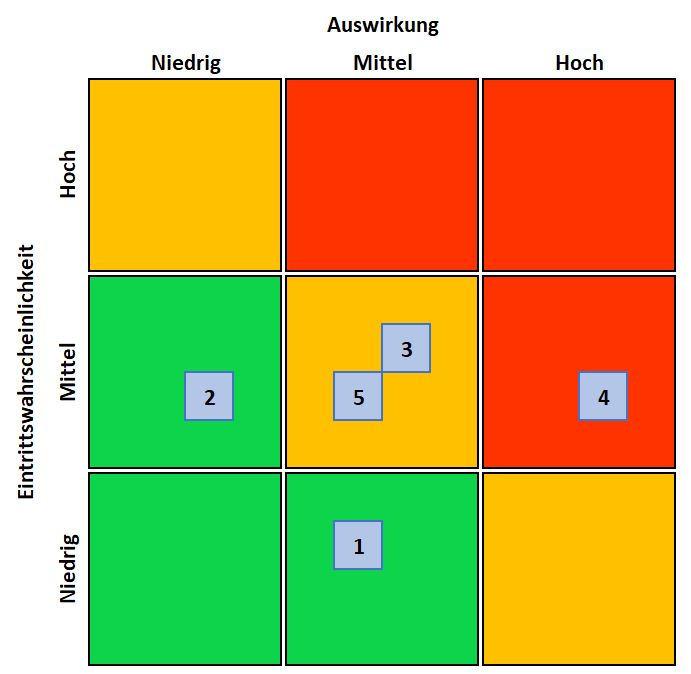
\includegraphics[scale=0.6]{Risikoanalyse.jpg}
\caption{Risiken}
\label{fig:Risk}
\end{figure} 

\begin{table}[H]
\centering
\begin{tabular}{p{1cm}p{6cm}p{9cm}}
\hline
\rowcolor{heading} \textbf{Nr.} & \textbf{Beschreibung} & \textbf{Massnahmen zur Problemlösung} \\\hline
1 & Der Terminplan kann nicht eingehalten werden & - Zeitplan anpassen \newline - Experten informieren und nach einer Lösung suchen \\\hline
2 & Ausfall durch Unfall & Experten informieren und nach einer Lösung suchen  \\\hline
3 & Technische Umsetzungsprobleme & - Informieren der Experten \newline - Hilfe der Experten einholen \newline - Alternative Lösung umsetzen \\\hline
4 & Defekte Hardware (Switch, Netzteil) & Hardware muss umgehend neu beschafft werden  \\\hline
5 & Softwarefehler & Patches einspielen, Kontakt mit Lieferanten aufnehmen  \\\hline
\end{tabular}
\caption{Risiken}
\end{table}


